\chapter{Haydée}

Scarcely had the count’s horses cleared the angle of the boulevard,
when Albert, turning towards the count, burst into a loud fit of
laughter—much too loud in fact not to give the idea of its being rather
forced and unnatural.

“Well,” said he, “I will ask you the same question which Charles IX.
put to Catherine de’ Medici, after the massacre of Saint Bartholomew:
‘How have I played my little part?’”

“To what do you allude?” asked Monte Cristo.

“To the installation of my rival at M. Danglars’.”

“What rival?”

“\textit{Ma foi!} what rival? Why, your protégé, M. Andrea Cavalcanti!”

“Ah, no joking, viscount, if you please; I do not patronize M.
Andrea—at least, not as concerns M. Danglars.”

“And you would be to blame for not assisting him, if the young man
really needed your help in that quarter, but, happily for me, he can
dispense with it.”

“What, do you think he is paying his addresses?”

“I am certain of it; his languishing looks and modulated tones when
addressing Mademoiselle Danglars fully proclaim his intentions. He
aspires to the hand of the proud Eugénie.”

“What does that signify, so long as they favor your suit?”

“But it is not the case, my dear count: on the contrary. I am repulsed
on all sides.”

“What!”

“It is so indeed; Mademoiselle Eugénie scarcely answers me, and
Mademoiselle d’Armilly, her confidant, does not speak to me at all.”

“But the father has the greatest regard possible for you,” said Monte
Cristo.

“He? Oh, no, he has plunged a thousand daggers into my heart,
tragedy-weapons, I own, which instead of wounding sheathe their points
in their own handles, but daggers which he nevertheless believed to be
real and deadly.”

“Jealousy indicates affection.”

“True; but I am not jealous.”

“He is.”

“Of whom?—of Debray?”

“No, of you.”

“Of me? I will engage to say that before a week is past the door will
be closed against me.”

“You are mistaken, my dear viscount.”

“Prove it to me.”

“Do you wish me to do so?”

“Yes.”

“Well, I am charged with the commission of endeavoring to induce the
Comte de Morcerf to make some definite arrangement with the baron.”

“By whom are you charged?”

“By the baron himself.”

“Oh,” said Albert with all the cajolery of which he was capable. “You
surely will not do that, my dear count?”

“Certainly I shall, Albert, as I have promised to do it.”

“Well,” said Albert, with a sigh, “it seems you are determined to marry
me.”

“I am determined to try and be on good terms with everybody, at all
events,” said Monte Cristo. “But apropos of Debray, how is it that I
have not seen him lately at the baron’s house?”

“There has been a misunderstanding.”

“What, with the baroness?”

“No, with the baron.”

“Has he perceived anything?”

“Ah, that is a good joke!”

“Do you think he suspects?” said Monte Cristo with charming
artlessness.

“Where have you come from, my dear count?” said Albert.

“From Congo, if you will.”

“It must be farther off than even that.”

“But what do I know of your Parisian husbands?”

“Oh, my dear count, husbands are pretty much the same everywhere; an
individual husband of any country is a pretty fair specimen of the
whole race.”

“But then, what can have led to the quarrel between Danglars and
Debray? They seemed to understand each other so well,” said Monte
Cristo with renewed energy.

“Ah, now you are trying to penetrate into the mysteries of Isis, in
which I am not initiated. When M. Andrea Cavalcanti has become one of
the family, you can ask him that question.”

The carriage stopped.

“Here we are,” said Monte Cristo; “it is only half-past ten o’clock,
come in.”

“Certainly, I will.”

“My carriage shall take you back.”

“No, thank you; I gave orders for my \textit{coupé} to follow me.”

“There it is, then,” said Monte Cristo, as he stepped out of the
carriage. They both went into the house; the drawing-room was lighted
up—they went in there. “You will make tea for us, Baptistin,” said the
count. Baptistin left the room without waiting to answer, and in two
seconds reappeared, bringing on a tray, all that his master had
ordered, ready prepared, and appearing to have sprung from the ground,
like the repasts which we read of in fairy tales.

“Really, my dear count,” said Morcerf, “what I admire in you is, not so
much your riches, for perhaps there are people even wealthier than
yourself, nor is it only your wit, for Beaumarchais might have
possessed as much,—but it is your manner of being served, without any
questions, in a moment, in a second; it is as if they guessed what you
wanted by your manner of ringing, and made a point of keeping
everything you can possibly desire in constant readiness.”

“What you say is perhaps true; they know my habits. For instance, you
shall see; how do you wish to occupy yourself during tea-time?”

“\textit{Ma foi}, I should like to smoke.”

Monte Cristo took the gong and struck it once. In about the space of a
second a private door opened, and Ali appeared, bringing two chibouques
filled with excellent latakia.

“It is quite wonderful,” said Albert.

“Oh no, it is as simple as possible,” replied Monte Cristo. “Ali knows
I generally smoke while I am taking my tea or coffee; he has heard that
I ordered tea, and he also knows that I brought you home with me; when
I summoned him he naturally guessed the reason of my doing so, and as
he comes from a country where hospitality is especially manifested
through the medium of smoking, he naturally concludes that we shall
smoke in company, and therefore brings two chibouques instead of
one—and now the mystery is solved.”

“Certainly you give a most commonplace air to your explanation, but it
is not the less true that you——Ah, but what do I hear?” and Morcerf
inclined his head towards the door, through which sounds seemed to
issue resembling those of a guitar.

“\textit{Ma foi}, my dear viscount, you are fated to hear music this evening;
you have only escaped from Mademoiselle Danglars’ piano, to be attacked
by Haydée’s guzla.”

“Haydée—what an adorable name! Are there, then, really women who bear
the name of Haydée anywhere but in Byron’s poems?”

“Certainly there are. Haydée is a very uncommon name in France, but is
common enough in Albania and Epirus; it is as if you said, for example,
Chastity, Modesty, Innocence,—it is a kind of baptismal name, as you
Parisians call it.”

“Oh, that is charming,” said Albert, “how I should like to hear my
countrywomen called Mademoiselle Goodness, Mademoiselle Silence,
Mademoiselle Christian Charity! Only think, then, if Mademoiselle
Danglars, instead of being called Claire-Marie-Eugénie, had been named
Mademoiselle Chastity-Modesty-Innocence Danglars; what a fine effect
that would have produced on the announcement of her marriage!”

“Hush,” said the count, “do not joke in so loud a tone; Haydée may hear
you, perhaps.”

“And you think she would be angry?”

“No, certainly not,” said the count with a haughty expression.

“She is very amiable, then, is she not?” said Albert.

“It is not to be called amiability, it is her duty; a slave does not
dictate to a master.”

“Come; you are joking yourself now. Are there any more slaves to be had
who bear this beautiful name?”

“Undoubtedly.”

“Really, count, you do nothing, and have nothing like other people. The
slave of the Count of Monte Cristo! Why, it is a rank of itself in
France, and from the way in which you lavish money, it is a place that
must be worth a hundred thousand francs a year.”

“A hundred thousand francs! The poor girl originally possessed much
more than that; she was born to treasures in comparison with which
those recorded in the \textit{Thousand and One Nights} would seem but
poverty.”

“She must be a princess then.”

“You are right; and she is one of the greatest in her country too.”

“I thought so. But how did it happen that such a great princess became
a slave?”

“How was it that Dionysius the Tyrant became a schoolmaster? The
fortune of war, my dear viscount,—the caprice of fortune; that is the
way in which these things are to be accounted for.”

“And is her name a secret?”

“As regards the generality of mankind it is; but not for you, my dear
viscount, who are one of my most intimate friends, and on whose silence
I feel I may rely, if I consider it necessary to enjoin it—may I not do
so?”

“Certainly; on my word of honor.”

“You know the history of the Pasha of Yanina, do you not?”

“Of Ali Tepelini?\footnote[13]{Ali Pasha, “The Lion,” was born at Tepelini,
an Albanian village at the foot of the Klissoura Mountains, in 1741. By
diplomacy and success in arms he became almost supreme ruler of Albania,
Epirus, and adjacent territory. Having aroused the enmity of the Sultan,
he was proscribed and put to death by treachery in 1822, at the age of
eighty.—Ed.} Oh, yes; it was in his service that my father made his fortune.”

“True, I had forgotten that.”

\begin{figure}[ht]
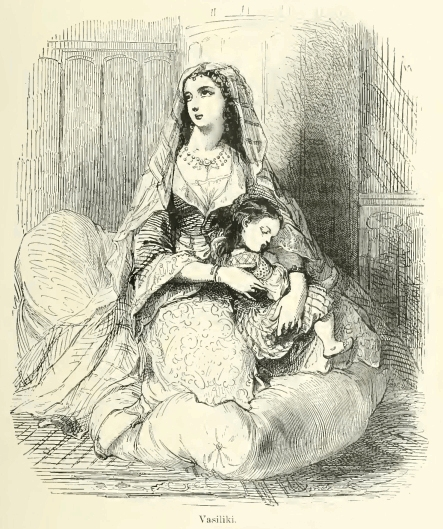
\includegraphics[width=\textwidth]{40062m.jpg}
\end{figure}

“Well, what is Haydée to Ali Tepelini?”

“Merely his daughter.”

“What? the daughter of Ali Pasha?”

“Of Ali Pasha and the beautiful Vasiliki.”

“And your slave?”

“\textit{Ma foi}, yes.”

“But how did she become so?”

“Why, simply from the circumstance of my having bought her one day, as
I was passing through the market at Constantinople.”

“Wonderful! Really, my dear count, you seem to throw a sort of magic
influence over all in which you are concerned; when I listen to you,
existence no longer seems reality, but a waking dream. Now, I am
perhaps going to make an imprudent and thoughtless request, but——”

“Say on.”

“But, since you go out with Haydée, and sometimes even take her to the
Opera——”

“Well?”

“I think I may venture to ask you this favor.”

“You may venture to ask me anything.”

“Well then, my dear count, present me to your princess.”

“I will do so; but on two conditions.”

“I accept them at once.”

“The first is, that you will never tell anyone that I have granted the
interview.”

“Very well,” said Albert, extending his hand; “I swear I will not.”

“The second is, that you will not tell her that your father ever served
hers.”

“I give you my oath that I will not.”

“Enough, viscount; you will remember those two vows, will you not? But
I know you to be a man of honor.”

The count again struck the gong. Ali reappeared. “Tell Haydée,” said
he, “that I will take coffee with her, and give her to understand that
I desire permission to present one of my friends to her.”

Ali bowed and left the room.

“Now, understand me,” said the count, “no direct questions, my dear
Morcerf; if you wish to know anything, tell me, and I will ask her.”

“Agreed.”

Ali reappeared for the third time, and drew back the tapestried hanging
which concealed the door, to signify to his master and Albert that they
were at liberty to pass on.

“Let us go in,” said Monte Cristo.

Albert passed his hand through his hair, and curled his moustache,
then, having satisfied himself as to his personal appearance, followed
the count into the room, the latter having previously resumed his hat
and gloves. Ali was stationed as a kind of advanced guard, and the door
was kept by the three French attendants, commanded by Myrtho.

Haydée was awaiting her visitors in the first room of her apartments,
which was the drawing-room. Her large eyes were dilated with surprise
and expectation, for it was the first time that any man, except Monte
Cristo, had been accorded an entrance into her presence. She was
sitting on a sofa placed in an angle of the room, with her legs crossed
under her in the Eastern fashion, and seemed to have made for herself,
as it were, a kind of nest in the rich Indian silks which enveloped
her. Near her was the instrument on which she had just been playing; it
was elegantly fashioned, and worthy of its mistress. On perceiving
Monte Cristo, she arose and welcomed him with a smile peculiar to
herself, expressive at once of the most implicit obedience and also of
the deepest love. Monte Cristo advanced towards her and extended his
hand, which she as usual raised to her lips.

\begin{figure}[ht]
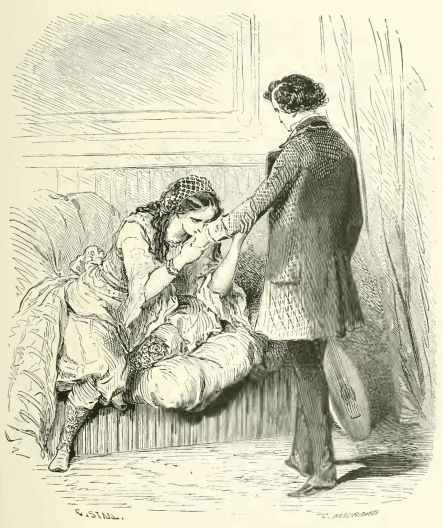
\includegraphics[width=\textwidth]{40064m.jpg}
\end{figure}

Albert had proceeded no farther than the door, where he remained rooted
to the spot, being completely fascinated by the sight of such
surpassing beauty, beheld as it was for the first time, and of which an
inhabitant of more northern climes could form no adequate idea.

“Whom do you bring?” asked the young girl in Romaic, of Monte Cristo;
“is it a friend, a brother, a simple acquaintance, or an enemy.”

“A friend,” said Monte Cristo in the same language.

“What is his name?”

“Count Albert; it is the same man whom I rescued from the hands of the
banditti at Rome.”

“In what language would you like me to converse with him?”

Monte Cristo turned to Albert. “Do you know modern Greek,” asked he.

“Alas! no,” said Albert; “nor even ancient Greek, my dear count; never
had Homer or Plato a more unworthy scholar than myself.”

“Then,” said Haydée, proving by her remark that she had quite
understood Monte Cristo’s question and Albert’s answer, “then I will
speak either in French or Italian, if my lord so wills it.”

Monte Cristo reflected one instant. “You will speak in Italian,” said
he.

Then, turning towards Albert,—“It is a pity you do not understand
either ancient or modern Greek, both of which Haydée speaks so
fluently; the poor child will be obliged to talk to you in Italian,
which will give you but a very false idea of her powers of
conversation.”

The count made a sign to Haydée to address his visitor. “Sir,” she said
to Morcerf, “you are most welcome as the friend of my lord and master.”
This was said in excellent Tuscan, and with that soft Roman accent
which makes the language of Dante as sonorous as that of Homer. Then,
turning to Ali, she directed him to bring coffee and pipes, and when he
had left the room to execute the orders of his young mistress she
beckoned Albert to approach nearer to her. Monte Cristo and Morcerf
drew their seats towards a small table, on which were arranged music,
drawings, and vases of flowers. Ali then entered bringing coffee and
chibouques; as to M. Baptistin, this portion of the building was
interdicted to him. Albert refused the pipe which the Nubian offered
him.

“Oh, take it—take it,” said the count; “Haydée is almost as civilized
as a Parisian; the smell of a Havana is disagreeable to her, but the
tobacco of the East is a most delicious perfume, you know.”

Ali left the room. The cups of coffee were all prepared, with the
addition of sugar, which had been brought for Albert. Monte Cristo and
Haydée took the beverage in the original Arabian manner, that is to
say, without sugar. Haydée took the porcelain cup in her little slender
fingers and conveyed it to her mouth with all the innocent artlessness
of a child when eating or drinking something which it likes. At this
moment two women entered, bringing salvers filled with ices and
sherbet, which they placed on two small tables appropriated to that
purpose.

“My dear host, and you, signora,” said Albert, in Italian, “excuse my
apparent stupidity. I am quite bewildered, and it is natural that it
should be so. Here I am in the heart of Paris; but a moment ago I heard
the rumbling of the omnibuses and the tinkling of the bells of the
lemonade-sellers, and now I feel as if I were suddenly transported to
the East; not such as I have seen it, but such as my dreams have
painted it. Oh, signora, if I could but speak Greek, your conversation,
added to the fairy-scene which surrounds me, would furnish an evening
of such delight as it would be impossible for me ever to forget.”

“I speak sufficient Italian to enable me to converse with you, sir,”
said Haydée quietly; “and if you like what is Eastern, I will do my
best to secure the gratification of your tastes while you are here.”

“On what subject shall I converse with her?” said Albert, in a low tone
to Monte Cristo.

“Just what you please; you may speak of her country and of her youthful
reminiscences, or if you like it better you can talk of Rome, Naples,
or Florence.”

“Oh,” said Albert, “it is of no use to be in the company of a Greek if
one converses just in the same style as with a Parisian; let me speak
to her of the East.”

“Do so then, for of all themes which you could choose that will be the
most agreeable to her taste.”

Albert turned towards Haydée. “At what age did you leave Greece,
signora?” asked he.

“I left it when I was but five years old,” replied Haydée.

“And have you any recollection of your country?”

“When I shut my eyes and think, I seem to see it all again. The mind
can see as well as the body. The body forgets sometimes; but the mind
always remembers.”

“And how far back into the past do your recollections extend?”

“I could scarcely walk when my mother, who was called Vasiliki, which
means royal,” said the young girl, tossing her head proudly, “took me
by the hand, and after putting in our purse all the money we possessed,
we went out, both covered with veils, to solicit alms for the
prisoners, saying, ‘He who giveth to the poor lendeth to the Lord.’
Then when our purse was full we returned to the palace, and without
saying a word to my father, we sent it to the convent, where it was
divided amongst the prisoners.”

“And how old were you at that time?”

“I was three years old,” said Haydée.

“Then you remember everything that went on about you from the time when
you were three years old?” said Albert.

“Everything.”

“Count,” said Albert, in a low tone to Monte Cristo, “do allow the
signora to tell me something of her history. You prohibited my
mentioning my father’s name to her, but perhaps she will allude to him
of her own accord in the course of the recital, and you have no idea
how delighted I should be to hear our name pronounced by such beautiful
lips.”

Monte Cristo turned to Haydée, and with an expression of countenance
which commanded her to pay the most implicit attention to his words, he
said in Greek, “Πατρὸς μὲν ἄτην μήζε τὸ ὄνομα προδότου καὶ προδοσίαν
εἰπὲ ἡμῖν,”—that is, “Tell us the fate of your father; but neither the
name of the traitor nor the treason.” Haydée sighed deeply, and a shade
of sadness clouded her beautiful brow.

“What are you saying to her?” said Morcerf in an undertone.

“I again reminded her that you were a friend, and that she need not
conceal anything from you.”

“Then,” said Albert, “this pious pilgrimage in behalf of the prisoners
was your first remembrance; what is the next?”

“Oh, then I remember as if it were but yesterday sitting under the
shade of some sycamore-trees, on the borders of a lake, in the waters
of which the trembling foliage was reflected as in a mirror. Under the
oldest and thickest of these trees, reclining on cushions, sat my
father; my mother was at his feet, and I, childlike, amused myself by
playing with his long white beard which descended to his girdle, or
with the diamond-hilt of the scimitar attached to his girdle. Then from
time to time there came to him an Albanian who said something to which
I paid no attention, but which he always answered in the same tone of
voice, either ‘Kill,’ or ‘Pardon.’”

“It is very strange,” said Albert, “to hear such words proceed from the
mouth of anyone but an actress on the stage, and one needs constantly
to be saying to one’s self, ‘This is no fiction, it is all reality,’ in
order to believe it. And how does France appear in your eyes,
accustomed as they have been to gaze on such enchanted scenes?”

“I think it is a fine country,” said Haydée, “but I see France as it
really is, because I look on it with the eyes of a woman; whereas my
own country, which I can only judge of from the impression produced on
my childish mind, always seems enveloped in a vague atmosphere, which
is luminous or otherwise, according as my remembrances of it are sad or
joyous.”

“So young,” said Albert, forgetting at the moment the Count’s command
that he should ask no questions of the slave herself, “is it possible
that you can have known what suffering is except by name?”

Haydée turned her eyes towards Monte Cristo, who, making at the same
time some imperceptible sign, murmured:

“Εἰπέ—speak.”

“Nothing is ever so firmly impressed on the mind as the memory of our
early childhood, and with the exception of the two scenes I have just
described to you, all my earliest reminiscences are fraught with
deepest sadness.”

\begin{figure}[ht]
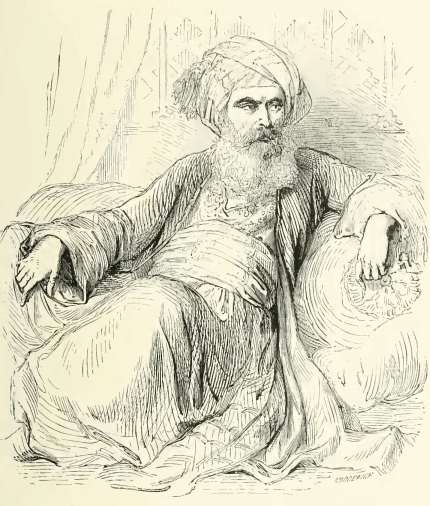
\includegraphics[width=\textwidth]{40068m.jpg}
\end{figure}

“Speak, speak, signora,” said Albert, “I am listening with the most
intense delight and interest to all you say.”

Haydée answered his remark with a melancholy smile. “You wish me, then,
to relate the history of my past sorrows?” said she.

“I beg you to do so,” replied Albert.

“Well, I was but four years old when one night I was suddenly awakened
by my mother. We were in the palace of Yanina; she snatched me from the
cushions on which I was sleeping, and on opening my eyes I saw hers
filled with tears. She took me away without speaking. When I saw her
weeping I began to cry too. ‘Hush, child!’ said she. At other times in
spite of maternal endearments or threats, I had with a child’s caprice
been accustomed to indulge my feelings of sorrow or anger by crying as
much as I felt inclined; but on this occasion there was an intonation
of such extreme terror in my mother’s voice when she enjoined me to
silence, that I ceased crying as soon as her command was given. She
bore me rapidly away.

“I saw then that we were descending a large staircase; around us were
all my mother’s servants carrying trunks, bags, ornaments, jewels,
purses of gold, with which they were hurrying away in the greatest
distraction.

“Behind the women came a guard of twenty men armed with long guns and
pistols, and dressed in the costume which the Greeks have assumed since
they have again become a nation. You may imagine there was something
startling and ominous,” said Haydée, shaking her head and turning pale
at the mere remembrance of the scene, “in this long file of slaves and
women only half-aroused from sleep, or at least so they appeared to me,
who was myself scarcely awake. Here and there on the walls of the
staircase, were reflected gigantic shadows, which trembled in the
flickering light of the pine-torches till they seemed to reach to the
vaulted roof above.

“‘Quick!’ said a voice at the end of the gallery. This voice made
everyone bow before it, resembling in its effect the wind passing over
a field of wheat, by its superior strength forcing every ear to yield
obeisance. As for me, it made me tremble. This voice was that of my
father. He came last, clothed in his splendid robes and holding in his
hand the carbine which your emperor presented him. He was leaning on
the shoulder of his favorite Selim, and he drove us all before him, as
a shepherd would his straggling flock. My father,” said Haydée, raising
her head, “was that illustrious man known in Europe under the name of
Ali Tepelini, pasha of Yanina, and before whom Turkey trembled.”

Albert, without knowing why, started on hearing these words pronounced
with such a haughty and dignified accent; it appeared to him as if
there was something supernaturally gloomy and terrible in the
expression which gleamed from the brilliant eyes of Haydée at this
moment; she appeared like a Pythoness evoking a spectre, as she
recalled to his mind the remembrance of the fearful death of this man,
to the news of which all Europe had listened with horror.

“Soon,” said Haydée, “we halted on our march, and found ourselves on
the borders of a lake. My mother pressed me to her throbbing heart, and
at the distance of a few paces I saw my father, who was glancing
anxiously around. Four marble steps led down to the water’s edge, and
below them was a boat floating on the tide.

\begin{figure}[ht]
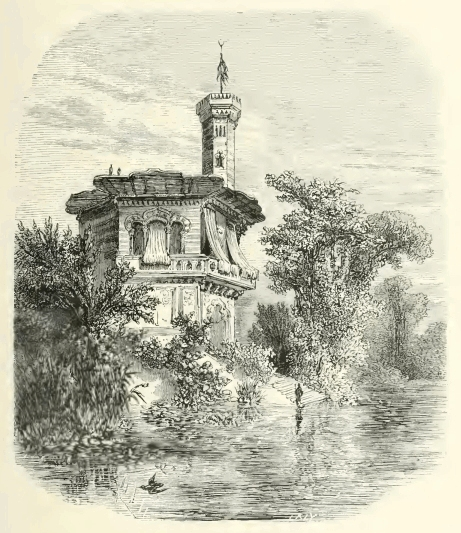
\includegraphics[width=\textwidth]{40070m.jpg}
\end{figure}

“From where we stood I could see in the middle of the lake a large
blank mass; it was the kiosk to which we were going. This kiosk
appeared to me to be at a considerable distance, perhaps on account of
the darkness of the night, which prevented any object from being more
than partially discerned. We stepped into the boat. I remember well
that the oars made no noise whatever in striking the water, and when I
leaned over to ascertain the cause I saw that they were muffled with
the sashes of our Palikares.14 Besides the rowers, the boat contained
only the women, my father, mother, Selim, and myself. The Palikares had
remained on the shore of the lake, ready to cover our retreat; they
were kneeling on the lowest of the marble steps, and in that manner
intended making a rampart of the three others, in case of pursuit. Our
bark flew before the wind. ‘Why does the boat go so fast?’ asked I of
my mother.

“‘Silence, child! Hush, we are flying!’ I did not understand. Why
should my father fly?—he, the all-powerful—he, before whom others were
accustomed to fly—he, who had taken for his device,

\begin{quote}
{\small‘They hate me; then they fear me!’}
\end{quote}

“It was, indeed, a flight which my father was trying to effect. I have
been told since that the garrison of the castle of Yanina, fatigued
with long service——”

Here Haydée cast a significant glance at Monte Cristo, whose eyes had
been riveted on her countenance during the whole course of her
narrative. The young girl then continued, speaking slowly, like a
person who is either inventing or suppressing some feature of the
history which he is relating.

“You were saying, signora,” said Albert, who was paying the most
implicit attention to the recital, “that the garrison of Yanina,
fatigued with long service——”

“Had treated with the Seraskier15 Kourchid, who had been sent by the
sultan to gain possession of the person of my father; it was then that
Ali Tepelini—after having sent to the sultan a French officer in whom
he reposed great confidence—resolved to retire to the asylum which he
had long before prepared for himself, and which he called
\textit{kataphygion}, or the refuge.”

“And this officer,” asked Albert, “do you remember his name, signora?”

Monte Cristo exchanged a rapid glance with the young girl, which was
quite unperceived by Albert.

“No,” said she, “I do not remember it just at this moment; but if it
should occur to me presently, I will tell you.”

Albert was on the point of pronouncing his father’s name, when Monte
Cristo gently held up his finger in token of reproach; the young man
recollected his promise, and was silent.

“It was towards this kiosk that we were rowing. A ground floor,
ornamented with arabesques, bathing its terraces in the water, and
another floor, looking on the lake, was all which was visible to the
eye. But beneath the ground floor, stretching out into the island, was
a large subterranean cavern, to which my mother, myself, and the women
were conducted. In this place were together 60,000 pouches and 200
barrels; the pouches contained 25,000,000 of money in gold, and the
barrels were filled with 30,000 pounds of gunpowder.

“Near the barrels stood Selim, my father’s favorite, whom I mentioned
to you just now. He stood watch day and night with a lance provided
with a lighted slowmatch in his hand, and he had orders to blow up
everything—kiosk, guards, women, gold, and Ali Tepelini himself—at the
first signal given by my father. I remember well that the slaves,
convinced of the precarious tenure on which they held their lives,
passed whole days and nights in praying, crying, and groaning. As for
me, I can never forget the pale complexion and black eyes of the young
soldier, and whenever the angel of death summons me to another world, I
am quite sure I shall recognize Selim. I cannot tell you how long we
remained in this state; at that period I did not even know what time
meant. Sometimes, but very rarely, my father summoned me and my mother
to the terrace of the palace; these were hours of recreation for me, as
I never saw anything in the dismal cavern but the gloomy countenances
of the slaves and Selim’s fiery lance. My father was endeavoring to
pierce with his eager looks the remotest verge of the horizon,
examining attentively every black speck which appeared on the lake,
while my mother, reclining by his side, rested her head on his
shoulder, and I played at his feet, admiring everything I saw with that
unsophisticated innocence of childhood which throws a charm round
objects insignificant in themselves, but which in its eyes are invested
with the greatest importance. The heights of Pindus towered above us;
the castle of Yanina rose white and angular from the blue waters of the
lake, and the immense masses of black vegetation which, viewed in the
distance, gave the idea of lichens clinging to the rocks, were in
reality gigantic fir-trees and myrtles.

“One morning my father sent for us; my mother had been crying all the
night, and was very wretched; we found the pasha calm, but paler than
usual. ‘Take courage, Vasiliki,’ said he; ‘today arrives the firman of
the master, and my fate will be decided. If my pardon be complete, we
shall return triumphant to Yanina; if the news be inauspicious, we must
fly this night.’—‘But supposing our enemy should not allow us to do
so?’ said my mother. ‘Oh, make yourself easy on that head,’ said Ali,
smiling; ‘Selim and his flaming lance will settle that matter. They
would be glad to see me dead, but they would not like themselves to die
with me.’

“My mother only answered by sighs to consolations which she knew did
not come from my father’s heart. She prepared the iced water which he
was in the habit of constantly drinking,—for since his sojourn at the
kiosk he had been parched by the most violent fever,—after which she
anointed his white beard with perfumed oil, and lighted his chibouque,
which he sometimes smoked for hours together, quietly watching the
wreaths of vapor that ascended in spiral clouds and gradually melted
away in the surrounding atmosphere. Presently he made such a sudden
movement that I was paralyzed with fear. Then, without taking his eyes
from the object which had first attracted his attention, he asked for
his telescope. My mother gave it him, and as she did so, looked whiter
than the marble against which she leaned. I saw my father’s hand
tremble. ‘A boat!—two!—three!’ murmured my, father;—‘four!’ He then
arose, seizing his arms and priming his pistols. ‘Vasiliki,’ said he to
my mother, trembling perceptibly, ‘the instant approaches which will
decide everything. In the space of half an hour we shall know the
emperor’s answer. Go into the cavern with Haydée.’—‘I will not quit
you,’ said Vasiliki; ‘if you die, my lord, I will die with you.’—‘Go to
Selim!’ cried my father. ‘Adieu, my lord,’ murmured my mother,
determining quietly to await the approach of death. ‘Take away
Vasiliki!’ said my father to his Palikares.

“As for me, I had been forgotten in the general confusion; I ran toward
Ali Tepelini; he saw me hold out my arms to him, and he stooped down
and pressed my forehead with his lips. Oh, how distinctly I remember
that kiss!—it was the last he ever gave me, and I feel as if it were
still warm on my forehead. On descending, we saw through the
lattice-work several boats which were gradually becoming more distinct
to our view. At first they appeared like black specks, and now they
looked like birds skimming the surface of the waves. During this time,
in the kiosk at my father’s feet, were seated twenty Palikares,
concealed from view by an angle of the wall and watching with eager
eyes the arrival of the boats. They were armed with their long guns
inlaid with mother-of-pearl and silver, and cartridges in great numbers
were lying scattered on the floor. My father looked at his watch, and
paced up and down with a countenance expressive of the greatest
anguish. This was the scene which presented itself to my view as I
quitted my father after that last kiss.

“My mother and I traversed the gloomy passage leading to the cavern.
Selim was still at his post, and smiled sadly on us as we entered. We
fetched our cushions from the other end of the cavern, and sat down by
Selim. In great dangers the devoted ones cling to each other; and,
young as I was, I quite understood that some imminent danger was
hanging over our heads.”

Albert had often heard—not from his father, for he never spoke on the
subject, but from strangers—the description of the last moments of the
vizier of Yanina; he had read different accounts of his death, but the
story seemed to acquire fresh meaning from the voice and expression of
the young girl, and her sympathetic accent and the melancholy
expression of her countenance at once charmed and horrified him.

As to Haydée, these terrible reminiscences seemed to have overpowered
her for a moment, for she ceased speaking, her head leaning on her hand
like a beautiful flower bowing beneath the violence of the storm; and
her eyes gazing on vacancy indicated that she was mentally
contemplating the green summit of the Pindus and the blue waters of the
lake of Yanina, which, like a magic mirror, seemed to reflect the
sombre picture which she sketched. Monte Cristo looked at her with an
indescribable expression of interest and pity.

“Go on, my child,” said the count in the Romaic language.

\begin{figure}[ht]
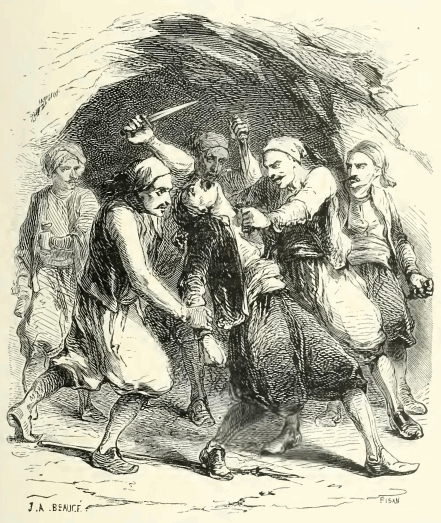
\includegraphics[width=\textwidth]{40074m.jpg}
\end{figure}

Haydée looked up abruptly, as if the sonorous tones of Monte Cristo’s
voice had awakened her from a dream; and she resumed her narrative.

“It was about four o’clock in the afternoon, and although the day was
brilliant out-of-doors, we were enveloped in the gloomy darkness of the
cavern. One single, solitary light was burning there, and it appeared
like a star set in a heaven of blackness; it was Selim’s flaming lance.
My mother was a Christian, and she prayed. Selim repeated from time to
time the sacred words: ‘God is great!’ However, my mother had still
some hope. As she was coming down, she thought she recognized the
French officer who had been sent to Constantinople, and in whom my
father placed so much confidence; for he knew that all the soldiers of
the French emperor were naturally noble and generous. She advanced some
steps towards the staircase, and listened. ‘They are approaching,’ said
she; ‘perhaps they bring us peace and liberty!’

“‘What do you fear, Vasiliki?’ said Selim, in a voice at once so gentle
and yet so proud. ‘If they do not bring us peace, we will give them
war; if they do not bring life, we will give them death.’ And he
renewed the flame of his lance with a gesture which made one think of
Dionysus of old Crete.\footnote[16]{The god of fruitfulness in Grecian
mythology. In Crete he was supposed to be slain in winter with the decay
of vegetation and to revive in the spring. Haydée’s learned reference is
to the behavior of an actor in the Dionysian festivals.—Ed.} But I,
being only a little child, was terrified by this undaunted courage, which
appeared to me both ferocious and senseless, and I recoiled with horror
from the idea of the frightful death amidst fire and flames which probably
awaited us.

“My mother experienced the same sensations, for I felt her tremble.
‘Mamma, mamma,’ said I, ‘are we really to be killed?’ And at the sound
of my voice the slaves redoubled their cries and prayers and
lamentations. ‘My child,’ said Vasiliki, ‘may God preserve you from
ever wishing for that death which today you so much dread!’ Then,
whispering to Selim, she asked what were her master’s orders. ‘If he
send me his poniard, it will signify that the emperor’s intentions are
not favorable, and I am to set fire to the powder; if, on the contrary,
he send me his ring, it will be a sign that the emperor pardons him,
and I am to extinguish the match and leave the magazine untouched.’—‘My
friend,’ said my mother, ‘when your master’s orders arrive, if it is
the poniard which he sends, instead of despatching us by that horrible
death which we both so much dread, you will mercifully kill us with
this same poniard, will you not?’—‘Yes, Vasiliki,’ replied Selim
tranquilly.

“Suddenly we heard loud cries; and, listening, discerned that they were
cries of joy. The name of the French officer who had been sent to
Constantinople resounded on all sides amongst our Palikares; it was
evident that he brought the answer of the emperor, and that it was
favorable.”

“And do you not remember the Frenchman’s name?” said Morcerf, quite
ready to aid the memory of the narrator. Monte Cristo made a sign to
him to be silent.

“I do not recollect it,” said Haydée.

“The noise increased; steps were heard approaching nearer and nearer;
they were descending the steps leading to the cavern. Selim made ready
his lance. Soon a figure appeared in the gray twilight at the entrance
of the cave, formed by the reflection of the few rays of daylight which
had found their way into this gloomy retreat. ‘Who are you?’ cried
Selim. ‘But whoever you may be, I charge you not to advance another
step.’—‘Long live the emperor!’ said the figure. ‘He grants a full
pardon to the Vizier Ali, and not only gives him his life, but restores
to him his fortune and his possessions.’ My mother uttered a cry of
joy, and clasped me to her bosom. ‘Stop,’ said Selim, seeing that she
was about to go out; ‘you see I have not yet received the
ring,’—‘True,’ said my mother. And she fell on her knees, at the same
time holding me up towards heaven, as if she desired, while praying to
God in my behalf, to raise me actually to his presence.”

And for the second time Haydée stopped, overcome by such violent
emotion that the perspiration stood upon her pale brow, and her stifled
voice seemed hardly able to find utterance, so parched and dry were her
throat and lips.

\begin{figure}[ht]
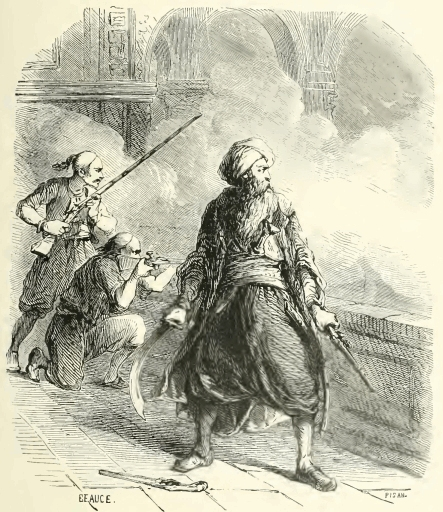
\includegraphics[width=\textwidth]{40076m.jpg}
\end{figure}

Monte Cristo poured a little iced water into a glass, and presented it
to her, saying with a mildness in which was also a shade of
command,—“Courage.”

Haydée dried her eyes, and continued:

“By this time our eyes, habituated to the darkness, had recognized the
messenger of the pasha,—it was a friend. Selim had also recognized him,
but the brave young man only acknowledged one duty, which was to obey.
‘In whose name do you come?’ said he to him. ‘I come in the name of our
master, Ali Tepelini.’—‘If you come from Ali himself,’ said Selim, ‘you
know what you were charged to remit to me?’—‘Yes,’ said the messenger,
‘and I bring you his ring.’ At these words he raised his hand above his
head, to show the token; but it was too far off, and there was not
light enough to enable Selim, where he was standing, to distinguish and
recognize the object presented to his view. ‘I do not see what you have
in your hand,’ said Selim. ‘Approach then,’ said the messenger, ‘or I
will come nearer to you, if you prefer it.’—‘I will agree to neither
one nor the other,’ replied the young soldier; ‘place the object which
I desire to see in the ray of light which shines there, and retire
while I examine it.’—‘Be it so,’ said the envoy; and he retired, after
having first deposited the token agreed on in the place pointed out to
him by Selim.

“Oh, how our hearts palpitated; for it did, indeed, seem to be a ring
which was placed there. But was it my father’s ring? that was the
question. Selim, still holding in his hand the lighted match, walked
towards the opening in the cavern, and, aided by the faint light which
streamed in through the mouth of the cave, picked up the token.

“‘It is well,’ said he, kissing it; ‘it is my master’s ring!’ And
throwing the match on the ground, he trampled on it and extinguished
it. The messenger uttered a cry of joy and clapped his hands. At this
signal four soldiers of the Seraskier Kourchid suddenly appeared, and
Selim fell, pierced by five blows. Each man had stabbed him separately,
and, intoxicated by their crime, though still pale with fear, they
sought all over the cavern to discover if there was any fear of fire,
after which they amused themselves by rolling on the bags of gold. At
this moment my mother seized me in her arms, and hurrying noiselessly
along numerous turnings and windings known only to ourselves, she
arrived at a private staircase of the kiosk, where was a scene of
frightful tumult and confusion. The lower rooms were entirely filled
with Kourchid’s troops; that is to say, with our enemies. Just as my
mother was on the point of pushing open a small door, we heard the
voice of the pasha sounding in a loud and threatening tone. My mother
applied her eye to the crack between the boards; I luckily found a
small opening which afforded me a view of the apartment and what was
passing within. ‘What do you want?’ said my father to some people who
were holding a paper inscribed with characters of gold. ‘What we want,’
replied one, ‘is to communicate to you the will of his highness. Do you
see this firman?’—‘I do,’ said my father. ‘Well, read it; he demands
your head.’

\begin{figure}[ht]
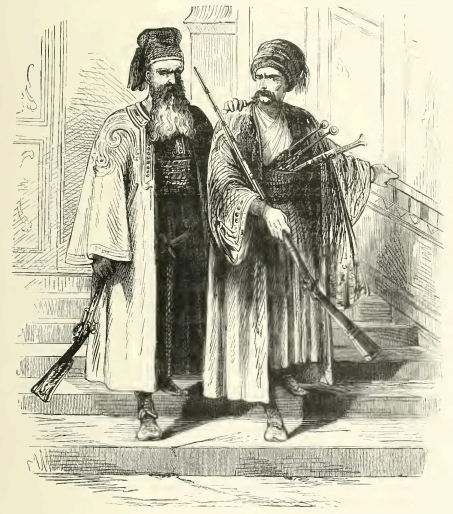
\includegraphics[width=\textwidth]{40078m.jpg}
\end{figure}

“My father answered with a loud laugh, which was more frightful than
even threats would have been, and he had not ceased when two reports of
a pistol were heard; he had fired them himself, and had killed two men.
The Palikares, who were prostrated at my father’s feet, now sprang up
and fired, and the room was filled with fire and smoke. At the same
instant the firing began on the other side, and the balls penetrated
the boards all round us. Oh, how noble did the grand vizier my father
look at that moment, in the midst of the flying bullets, his scimitar
in his hand, and his face blackened with the powder of his enemies! and
how he terrified them, even then, and made them fly before him! ‘Selim,
Selim!’ cried he, ‘guardian of the fire, do your duty!’—‘Selim is
dead,’ replied a voice which seemed to come from the depths of the
earth, ‘and you are lost, Ali!’ At the same moment an explosion was
heard, and the flooring of the room in which my father was sitting was
suddenly torn up and shivered to atoms—the troops were firing from
underneath. Three or four Palikares fell with their bodies literally
ploughed with wounds.

“My father howled aloud, plunged his fingers into the holes which the
balls had made, and tore up one of the planks entire. But immediately
through this opening twenty more shots were fired, and the flame,
rushing up like fire from the crater of a volcano, soon reached the
tapestry, which it quickly devoured. In the midst of all this frightful
tumult and these terrific cries, two reports, fearfully distinct,
followed by two shrieks more heartrending than all, froze me with
terror. These two shots had mortally wounded my father, and it was he
who had given utterance to these frightful cries. However, he remained
standing, clinging to a window. My mother tried to force the door, that
she might go and die with him, but it was fastened on the inside. All
around him were lying the Palikares, writhing in convulsive agonies,
while two or three who were only slightly wounded were trying to escape
by springing from the windows. At this crisis the whole flooring
suddenly gave way, my father fell on one knee, and at the same moment
twenty hands were thrust forth, armed with sabres, pistols, and
poniards—twenty blows were instantaneously directed against one man,
and my father disappeared in a whirlwind of fire and smoke kindled by
these demons, and which seemed like hell itself opening beneath his
feet. I felt myself fall to the ground, my mother had fainted.”

Haydée’s arms fell by her side, and she uttered a deep groan, at the
same time looking towards the count as if to ask if he were satisfied
with her obedience to his commands.

Monte Cristo arose and approached her, took her hand, and said to her
in Romaic:

“Calm yourself, my dear child, and take courage in remembering that
there is a God who will punish traitors.”

“It is a frightful story, count,” said Albert, terrified at the
paleness of Haydée’s countenance, “and I reproach myself now for having
been so cruel and thoughtless in my request.”

“Oh, it is nothing,” said Monte Cristo. Then, patting the young girl on
the head, he continued, “Haydée is very courageous, and she sometimes
even finds consolation in the recital of her misfortunes.”

“Because, my lord,” said Haydée eagerly, “my miseries recall to me the
remembrance of your goodness.”

Albert looked at her with curiosity, for she had not yet related what
he most desired to know,—how she had become the slave of the count.
Haydée saw at a glance the same expression pervading the countenances
of her two auditors; she continued:

“When my mother recovered her senses we were before the seraskier.
‘Kill,’ said she, ‘but spare the honor of the widow of Ali.’—‘It is not
to me to whom you must address yourself,’ said Kourchid.

“‘To whom, then?’—‘To your new master.’

“‘Who and where is he?’—‘He is here.’

“And Kourchid pointed out one who had more than any contributed to the
death of my father,” said Haydée, in a tone of chastened anger.

“Then,” said Albert, “you became the property of this man?”

“No,” replied Haydée, “he did not dare to keep us, so we were sold to
some slave-merchants who were going to Constantinople. We traversed
Greece, and arrived half dead at the imperial gates. They were
surrounded by a crowd of people, who opened a way for us to pass, when
suddenly my mother, having looked closely at an object which was
attracting their attention, uttered a piercing cry and fell to the
ground, pointing as she did so to a head which was placed over the
gates, and beneath which were inscribed these words:

‘\textit{This is the head of Ali Tepelini, Pasha of Yanina.}’

“I cried bitterly, and tried to raise my mother from the earth, but she
was dead! I was taken to the slave-market, and was purchased by a rich
Armenian. He caused me to be instructed, gave me masters, and when I
was thirteen years of age he sold me to the Sultan Mahmoud.”

“Of whom I bought her,” said Monte Cristo, “as I told you, Albert, with
the emerald which formed a match to the one I had made into a box for
the purpose of holding my hashish pills.”

“Oh, you are good, you are great, my lord!” said Haydée, kissing the
count’s hand, “and I am very fortunate in belonging to such a master!”

Albert remained quite bewildered with all that he had seen and heard.

“Come, finish your cup of coffee,” said Monte Cristo; “the history is
ended.”
